 \appendix
 \section{Proof of NP-completeness for Enforcing Isolation Policies} \label{sec:isolationNP}
 We show that the graph 3-coloring problem, which is NP-complete reduces to the enforcement problem for
 reachability and isolation policies. The latter is also in NP, so after the reduction we 
 can conclude that it is also NP-complete.

Let $G=(V,E)$ be an instance of the graph 3-coloring problem.
The graph $G$ admits a 3-coloring if there exists a function 
$f:G\mapsto \{R,G,B\}$ such that for every edge $(v1,v2)\in E$,
$f(v_1)\neq f(v_2)$.

We now show how to construct a topology $T=(S,L)$ and a corresponding set of policies $P$ that can be 
enforced iff $G$ admits 3-coloring.
The topology $T$ is the one depicted in  \cref{fig:swtopo}.
The set of flows is $V$, $v \in V$ we add a reachability policy $s >> d$ on the flow $v$.
For each edge $(v1,v2)\in E$ we add an isolation policy $v_1||v_2$.
 \begin{figure}[H] 
 	\centering
 	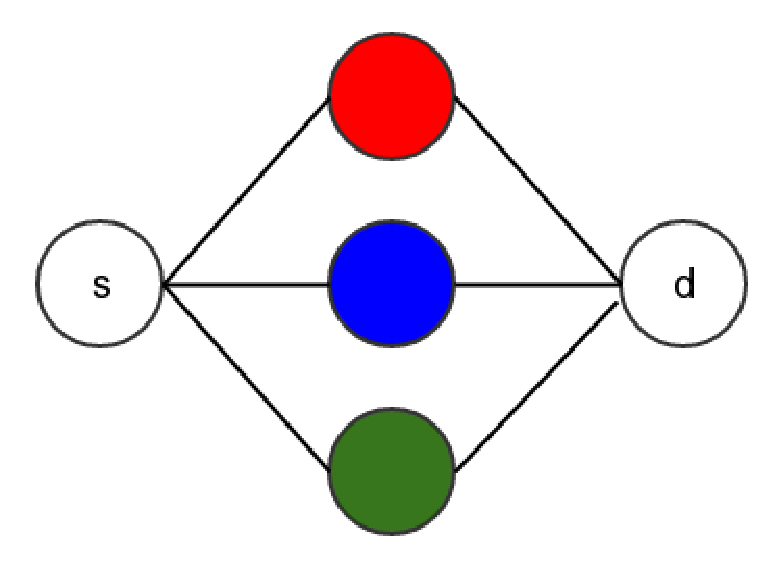
\includegraphics[width=0.7\columnwidth]{figures/color_topo.eps}
 	\caption{The switch topology $T$. All circles represent switches and all reachability policies are $s$ to $d$}
 	\label{fig:swtopo}
 \end{figure}
We not prove that if the policy can enforced $G$ admits 3-coloring.
If the policy is enforced, we have a path from $s$ to $d$ for each flow/vertex $v$.
We can set $f(v)$ to the color of the corresponding middle-switch being crossed.
Since for every $(v1,v2)\in E$ the two flows for $v_1$ and $v_2$ cannot share any edge,
they must have crossed two middle-switches with different colors and $f$ is a correct 3-coloring.
The other direction of the proof is analogous.

 
% \subsection{Enforcement of Waypoint Policies}
% Given a undirected graph $G={V,E}$. Let us assume there exists an polynomial-time algorithm to compute the reachability paths satisfying the policies of the following types on the graph : \\
% \begin{itemize} 
% 	\item \textbf{P1} : $v_1 >> v_2 \Rightarrow$ There exists a path from $v_1$ to $v_2$ satisfying all input policies. A property of the path is that it does not have repeat a vertex (no forwarding loops).
% 	\item \textbf{P2} : $v_1 >> W >> v_2 \Rightarrow$ The path from $v_1$ to $v_2$  should pass through the vertices in the set $W$ in any order, without repeating a vertex.
% \end{itemize}
% \textbf{Reduction of Hamiltonian Cycle Problem} : Given a undirected graph $G={V,E}$, find $v \in V$ such that the degree of $v$ is the minimum in the graph (Will work for any vertex actually). If a Hamiltonian cycle is present in the graph, it will have the vertex $v$ in the cycle, and one of the edges from $v$.  \\
% Lets take a $n \in Neighbours(v)$. Let the input policies to our algorithm be : 
% \begin{itemize}
% 	\item \textbf{P4} : $v >> W >> n$ where $W = V - \{v,n\} $ 
% \end{itemize}
%P4 cimputes a simple path from $v$ to $n$ which passes through all the other vertices in the graph which is the Hamiltonian path problem. Since computing the Hamiltonian path is NP-hard, the problem of path computation for the waypoint policies as specified is NP-hard. 